\section{Our WCET analysis framework}
\label{sec:overview}

%\textcolor{red}{\bf TODO: Figure qui illustre le framework}

\begin{figure}[htbp] %  figure placement: here, top, bottom, or page
   \centering
   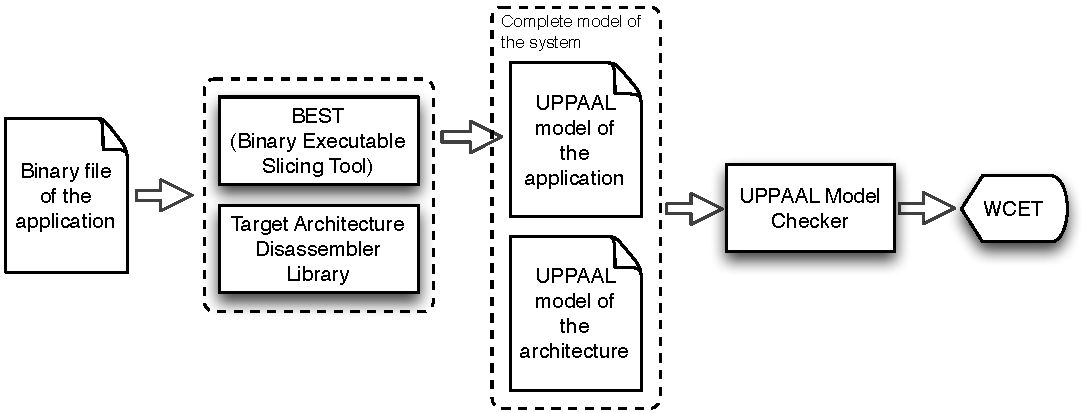
\includegraphics[width=\columnwidth]{fig/analysisFramework.pdf} 
   \caption{The UPPAAL model of the application is generated by the BEST tool, from the application binary file. This model is synchronized with the hand-written model of the architecture (that does not depend on the application considered). The WCET is then computed by model checking.}
   \label{fig:framework}
%   The binary file of the application to analyze is sliced and translated to an UPPAAL model. This model is synchronized with the model of the architecture. WCET is then computed by model checking.}
\end{figure}

As shown in figure \ref{fig:framework}, our analysis framework is built around two tools: BEST~\cite{wcet16_mangean} and UPPAAL~\cite{Larsen1997}.

BEST is a program slicing tool for binary code.
It is interfaced with a disassembler library for the target instruction set architecture (PowerPC 32-bit in this paper).
For each instruction of the program, the disassembler provides a set of semantics information including the opcode, the arguments, the type (branch or not), the set of used and defined registers, etc. % a textual "disassembled form", its address, ref. and def. registers, immediate arguments, if it is a branch, its conditionality, the kind of the test, if it is a direct or indirect branch, its target, if it is a memory load or store and more.
BEST uses this information to slice the program, with all the branch
instructions as the slice criterion.
The resulting sliced program contains all and only the instructions that have an
impact on the execution flow.
This sliced program is then used to produce a control flow graph where each instruction is tagged as either in or out of the slice.
From the set of instructions in the slice, the set of useful memory locations to analyze the control flow of the program is computed.
This information is then used to generate an UPPAAL model of the program (see section~\ref{sec:model:program}). The program slicing is a mandatory phase to limit the state space explosion problem.

%\textcolor{red}{The set of useful memory locations are part of the model, whereas the other are abstracted away.} % Soit je ne comprends pas, soit ce n'est pas le cas.
%Notice that BEST can also computes an UPPAAL model without slicing the program.
%In this case, all the memory locations used by the program are part of the model.

The second step consists in analyzing the system with UPPAAL.
UPPAAL is a model design and verification tool for networks of timed automata (NTA).
Timed automata (TA) are finite state automata augmented with real-valued clocks.
The values of these clocks all increase at the same rate.
Linear constraints on clocks can be used to guard transition, and clocks can be reset when a transition is taken.
In UPPAAL syntax, TA can use boolean and bounded integer variables.
These variables can be manipulated through functions specified in a language with a C-like syntax.
Moreover, TA can be synchronized over synchronous % Pas forcemment broadcast
 channels to form a NTA.

In our framework, we have developed a set of TA corresponding to the components of the microarchitecture. %: \textcolor{red}{memory, instruction cache, pipeline}. % Pas que et pas forcemment découpé comme ça. On peut mettre trois points de suspension ou ne pas enlever cette liste.
These components interact through global variables and synchronizations.
The corresponding models are briefly described in section~\ref{sec:model}.
The model of the program generated by BEST is synchronized with the models of the microarchitecture.
The resulting NTA models the whole system, hardware and software.
This model contains a specific clock reset one time only, at system startup. 
The model checker is then used to perform a symbolic exploration of the state space of the system and computes the maximal value reached by this clock over all paths.
  Our framework (BEST, UPPAAL models and script files) used to produce the experimental data are distributed in open-source\footnote{Available at
  \url{https://github.com/TrampolineRTOS/BEST}}.




%un tableau ?
% prediction | BTB | branch || cycles lost
% corret       | hit    |  taken   || 0
% …
% Bof, on est déjà à 9 pages :-P

%\subsubsection{Instruction path}
